\chapter{Simulating anisotropic diffusion in heterogeneous brain regions}
\label{chp:chp6}

In this chapter, we return to our model problem~\eqref{eq:diffusion}
and bring together the different tools and techniques introduced in
Chapters~\ref{chp:chp3} to \ref{chap:dti}. The computational domain will
be determined from T1-weighted data and divided into grey and white matter
subdomains, diffusion tensor imaging (DTI) data will be employed in the construction of the
heterogeneous and anisotropic diffusion tensor, and specific
sub regions, such as the hippocampus, will be selected to assess
site-specific clearance.

In practice, one should first address data and mesh resolution
issues. For instance, raw DTI data can exhibit rough transitions, as
well as noise. This is particularly true in the grey matter proximal
to cerebrospinal fluid (e.g.~Figures~\ref{fig:chp5:DTIfa} and
\ref{fig:chp5:freesurfer-parc} in Chapter \ref{chap:dti}). Here, we assume that 
the DTI data have been suitably smoothened and denoised for use in simulations. In
addition, we must ascertain a mesh resolution that is suitable to
provide reliable estimates of the spread and clearance of different
molecules, while avoiding the unnecessary computational costs
associated with over-resolving the mesh.

\section{Molecular diffusion in one dimension}
\label{sec:chp6:1D-tests}

\index{amyloid-beta}
To estimate the required spatial mesh resolution, the discrete
time step, and the time scale of solute clearance, it is useful to
first consider equation \eqref{eq:diffusion} in one dimension for different
molecules. Here, we consider the protein fragment amyloid-beta
(A$\beta$) associated with neurodegenerative
disease~\cite{iliff2012paravascular}, the tracer gadobutrol used in
glymphatic magnetic resonance imaging~\cite{ringstad2018brain}, and water. The
effective diffusion coefficient $D$ in brain tissue for each of these
molecules is estimated to be $6.2 \times 10^{-5}$ mm$^2$/s,
$1.3 \times 10^{-4}$ mm$^2$/s, and $1.1 \times 10^{-3}$ mm$^2$/s,
respectively~\cite{waters2010concentration,valnes2020apparent}.

\subsection{Analytical solution}
In one dimension and over the domain $(0, \infty)$, the parabolic
diffusion problem \eqref{eq:diffusion} with $u_0(x)=0$, $u(0, t) = 1$,
and $u(\infty, t) = 0$ allows for a simple analytic solution:
\begin{equation}
  \label{eq:analytical:1D}
  u(x,t) =  \mbox{erfc}(x / (2 \sqrt{D t})). 
\end{equation}

Figure~\ref{fig:chp6:analytics} shows solutions
of~\eqref{eq:analytical:1D} zoomed in on the (left) first 2 mm of the domain, 
and the (middle) first 10 mm after 9 hours, and (right) the first 10 mm after 24
hours. It is evident that diffusion is a slow process:
significant concentration changes occur within 2 mm of the boundary
after 9 hours; however, 1 cm away, the heavier molecules,
amyloid-beta and gadobutrol, still have concentrations near zero. The
source code for generating these plots is available in
\emp{mri2fem/chp6/analytical\_1D.py}.
\begin{figure}	
  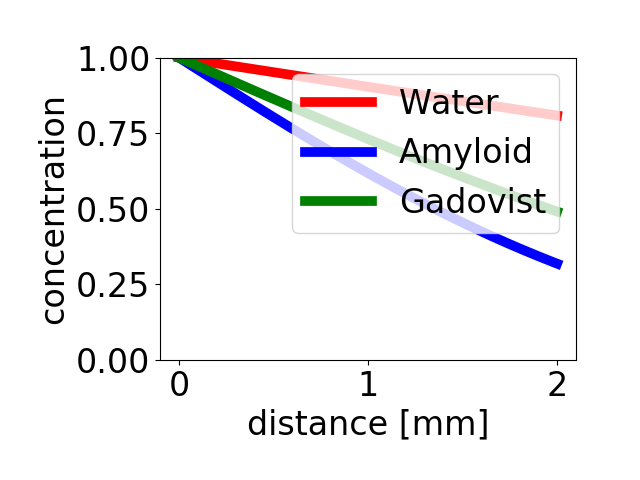
\includegraphics[width=0.32\textwidth]{./graphics/chp6/9hours_2mm_WAG}
  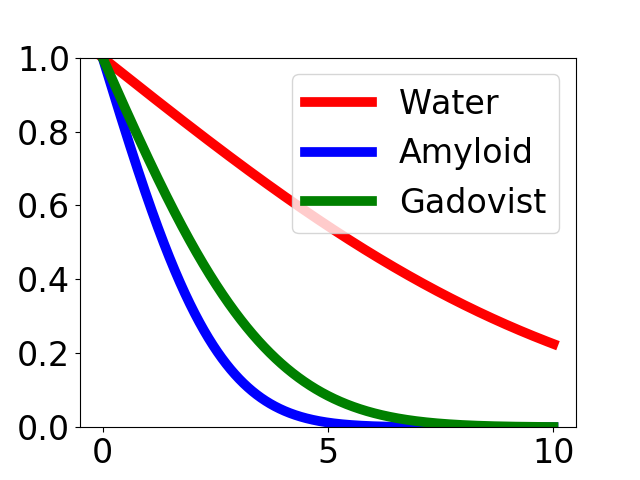
\includegraphics[width=0.32\textwidth]{./graphics/chp6/9hours_1cm_WAG}
  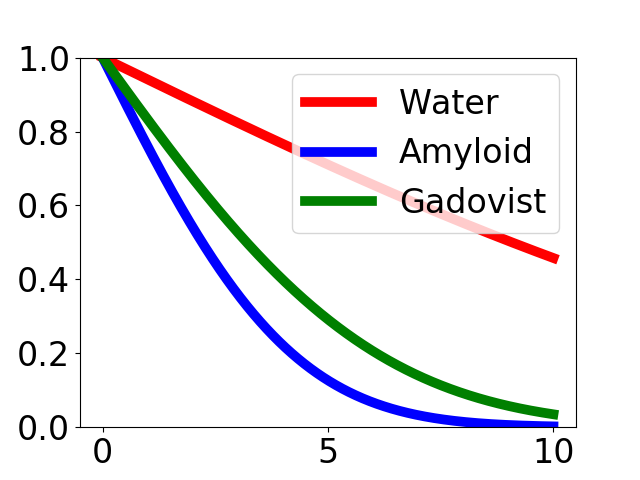
\includegraphics[width=0.32\textwidth]{./graphics/chp6/24hours_1cm_WAG}
  \caption{Diffusion according to \eqref{eq:analytical:1D}:
    concentration (arbitrary unit) versus distance from the
    source/left boundary  after 9 hours (left and middle) and
    after 24 hours (right).}
  \label{fig:chp6:analytics}
\end{figure}

\subsection{Numerical solution and handling numerical artifacts}
\index{mass lumping}
We next discretize \eqref{eq:diffusion} using the finite element
method (as described in Chapter~\ref{chp:chp3}). Note, however, that the
sharp change in the boundary versus initial conditions for our model
problem can lead to artificial oscillations in the numerical
solution. Such oscillations often diminish with refinement; they can
also be avoided through the use of monotonic or maximum principle
preserving schemes. Another common method, which we consider here, for
Galerkin finite element schemes is mass lumping (%
e.g.~\cite{langtangen2016solving}). We provide FEniCS-based source
code for the finite element solution of~\eqref{eq:diffusion} with and
without mass lumping in \emp{mri2fem/chp6/diffusion\_1D.py}. To use
this script, see, for example 
\terminal{\$ cd mri2fem/chp6 \\
\$ python3 diffusion\_1D.py -{}-help}
\begin{figure}	
\subfigure[$t=30$ minutes, standard Galerkin]{ 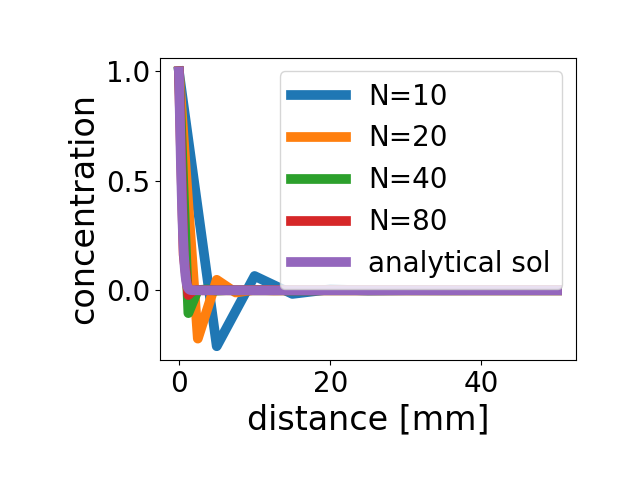
\includegraphics[width=0.49\textwidth]{./graphics/chp6/Amyloid_numerical_1D_L_max50_dt300_final1800_lumpednot.png}}
\subfigure[$t=30$ minutes, lumped mass matrix]{ 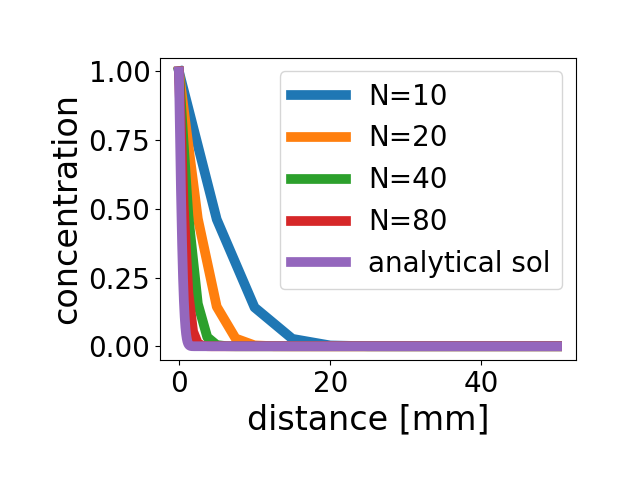
\includegraphics[width=0.49\textwidth]{./graphics/chp6/Amyloid_numerical_1D_L_max50_dt300_final1800_lumpedlumped.png}} \\
\subfigure[$t=9$ hours, standard Galerkin]{ 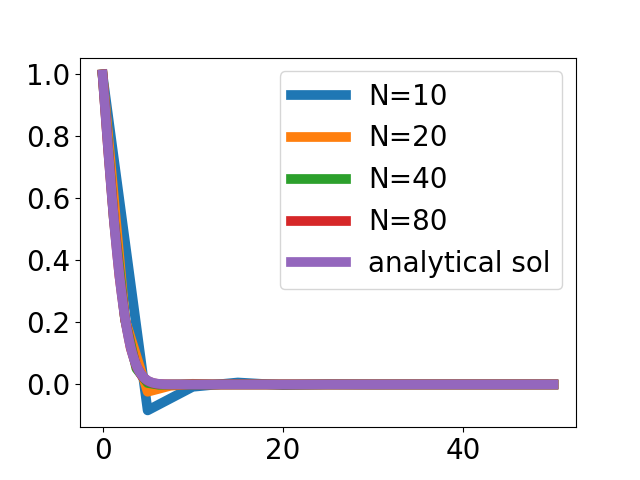
\includegraphics[width=0.49\textwidth]{./graphics/chp6/Amyloid_numerical_1D_L_max50_dt300_final32400_lumpednot.png}}
\subfigure[$t=9$ hours, lumped mass matrix]{ 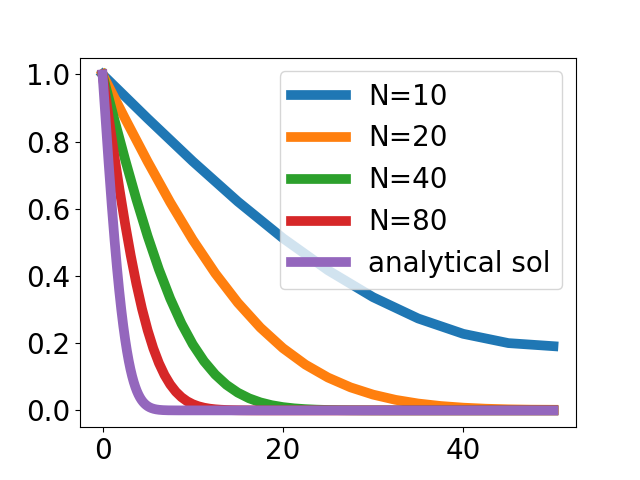
\includegraphics[width=0.49\textwidth]{./graphics/chp6/Amyloid_numerical_1D_L_max50_dt300_final32400_lumpedlumped.png}}
\caption{
  Comparison of standard Galerkin (left) and mass-lumped (right)
  finite element schemes of the diffusion
  equation~\eqref{eq:diffusion} in one dimension over $\Omega = (0, 50)$
  mm at different times.  }
\label{fig:chp6:numerics}
\end{figure}

The standard and mass-lumped finite element solutions are shown in
Figure~\ref{fig:chp6:numerics} at different times and with different
time steps. Early, for coarse resolutions ($N = 10$ or $N=20$), the
standard approach yields considerable nonphysical oscillations, whereas 
the mass-lumped solution (right) produces significant numerical
diffusion. However, in the longer term context, the standard Galerkin
scheme is clearly desirable: the former allows for a spatial
resolution of $N=10$ or $N=20$, whereas the latter requires $N=40$ or
$N=80$ to control the numerical diffusion. Essentially, the initial
error from the short-term Gibbs phenomena, that is, the discontinuous
initial data, is no match for the long-term regularizing effect of the
parabolic partial differential equation. Therefore, these early errors do not contribute much to the
long-term numerical solution.

In conclusion, these results suggest that, if we are interested in
long-term dynamics, a time step size of $\Delta t \approx$ 5 minutes with
a spatial resolution of $N=10$ or $N=20$, corresponding roughly to a
quasi-uniform mesh cell diameter of $0.25$ mm $\leq h \leq 0.5$ mm, is
a good starting target for the standard Galerkin approach in our three dimensional 
(3D) discretization. Conversely, a mesh size of $N = 80$, or $ h \approx
6.25\times 10^{-2}$ mm, is needed for the mass-lumped case.  This would
be a much more costly choice on a 3D mesh, and unnecessary if the
short-term dynamics do not need to be resolved.

\section{Anisotropic diffusion in 3D brain regions}

In this section, we consider simulations of gadobutrol diffusion 
and compute the average concentrations in different brain regions. In
particular, we begin with the following steps:
\begin{itemize}
\item
  We create a brain mesh with grey and white matter marked and
  ventricles removed and mark parcellation regions as described in
  Chapter~\ref{chp4:parcellations}. 
\item
  We filter and map our DTI data onto this geometry as described in 
  Chapter~\ref{chp5:sec:loading-dti-tensor}.
\item
  Using FEniCS, we implement a version of the diffusion simulation
  script presented in
  Chapter~\ref{sec:chp3:fenics-code-implementation} allowing for
  anisotropic diffusion and the computation of integrals over labelled
  regions.
\end{itemize}
In the numerical simulation, we represent the DTI data in the form of
a heterogeneous and anisotropic diffusion tensor field $D$. The FEniCS
code for setting up the diffusion tensor field reads 
\newpythonsnippet{chp6}{chp6-diffusion-mritracer.py}{35}{38}

\index{FEniCS!integrating over regions}
\noindent We compute the average amount of tracer in a labelled region by
integrating the concentration over the region and dividing by the
region's volume as follows (with the regions labelled 17 and 1035 as
examples):
\newpythonsnippet{chp6}{chp6-diffusion-mritracer.py}{151}{152}

\noindent The precise commands run are included in
\emp{mri2fem/chp6/all.sh}, and the script
\emp{mri2fem/chp6/chp6-diffusion-mritracer.py} gives the complete
FEniCS code.

\subsection{Regional distribution of gadobutrol}
We compute the average concentrations of gadobutrol diffusing in from
the brain's surface in regions 17 (hippocampus), 1035 (insula grey
matter), 3035 (insula white matter), 1028 (superior frontal grey
matter), and 3028 (superior frontal white matter).  Gadobutrol has a
diffusivity approximately twice that of amyloid-beta, and the
estimated mesh size and time step of the previous section should therefore apply
to this case as well.  The resulting curves are shown in
Figure~\ref{chp6:regions}, and the simulations are shown in
Figures~\ref{fig:chp6:numerics4}--\ref{fig:chp6:numerics5}. Note that, here, 
we consider the tracer distribution in certain regions as a
function of time; the distribution therefore starts at a low value and increases 
with time as the solute diffuses throughout the brain. Clearly, the
distribution of gadobutrol in the grey matter regions and hippocampus
are affected much more than in the white matter regions. This result is
expected since both the grey matter and hippocampus are
closer to the cerebrospinal fluid where, in our simulation, the gadobutrol
concentration is assumed to reside initially.  It is also observed
that the upper regions, that is, the superior frontal grey and white matter
(1028 and 3028, respectively), experience faster gadobutrol deposition
than the corresponding regions on the side of the brain.
\begin{figure}%[t]
  \centering
  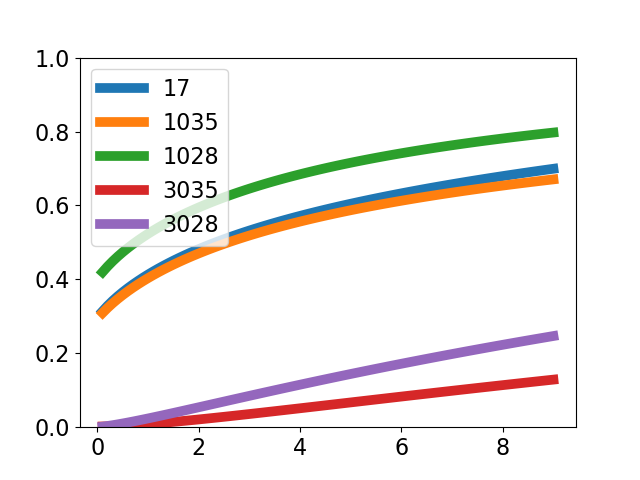
\includegraphics[width=0.7\textwidth]{./graphics/chp6/tracer_uniform_notlump_regions_64.png}
  \caption{Average concentration of gadobutrol (y-axis, arbitrary
    unit) versus time (x-axis, hours) in different brain regions: 17
    (hippocampus), 1035 (insula grey matter), 3035 (insula white
    matter), 1028 (superior frontal grey matter), and 3028
    (superior frontal white matter). Time step: 6 minutes, $N=64$ brain
    mesh (cf.~below).}
  \label{chp6:regions}
\end{figure}
%\begin{figure}	
%  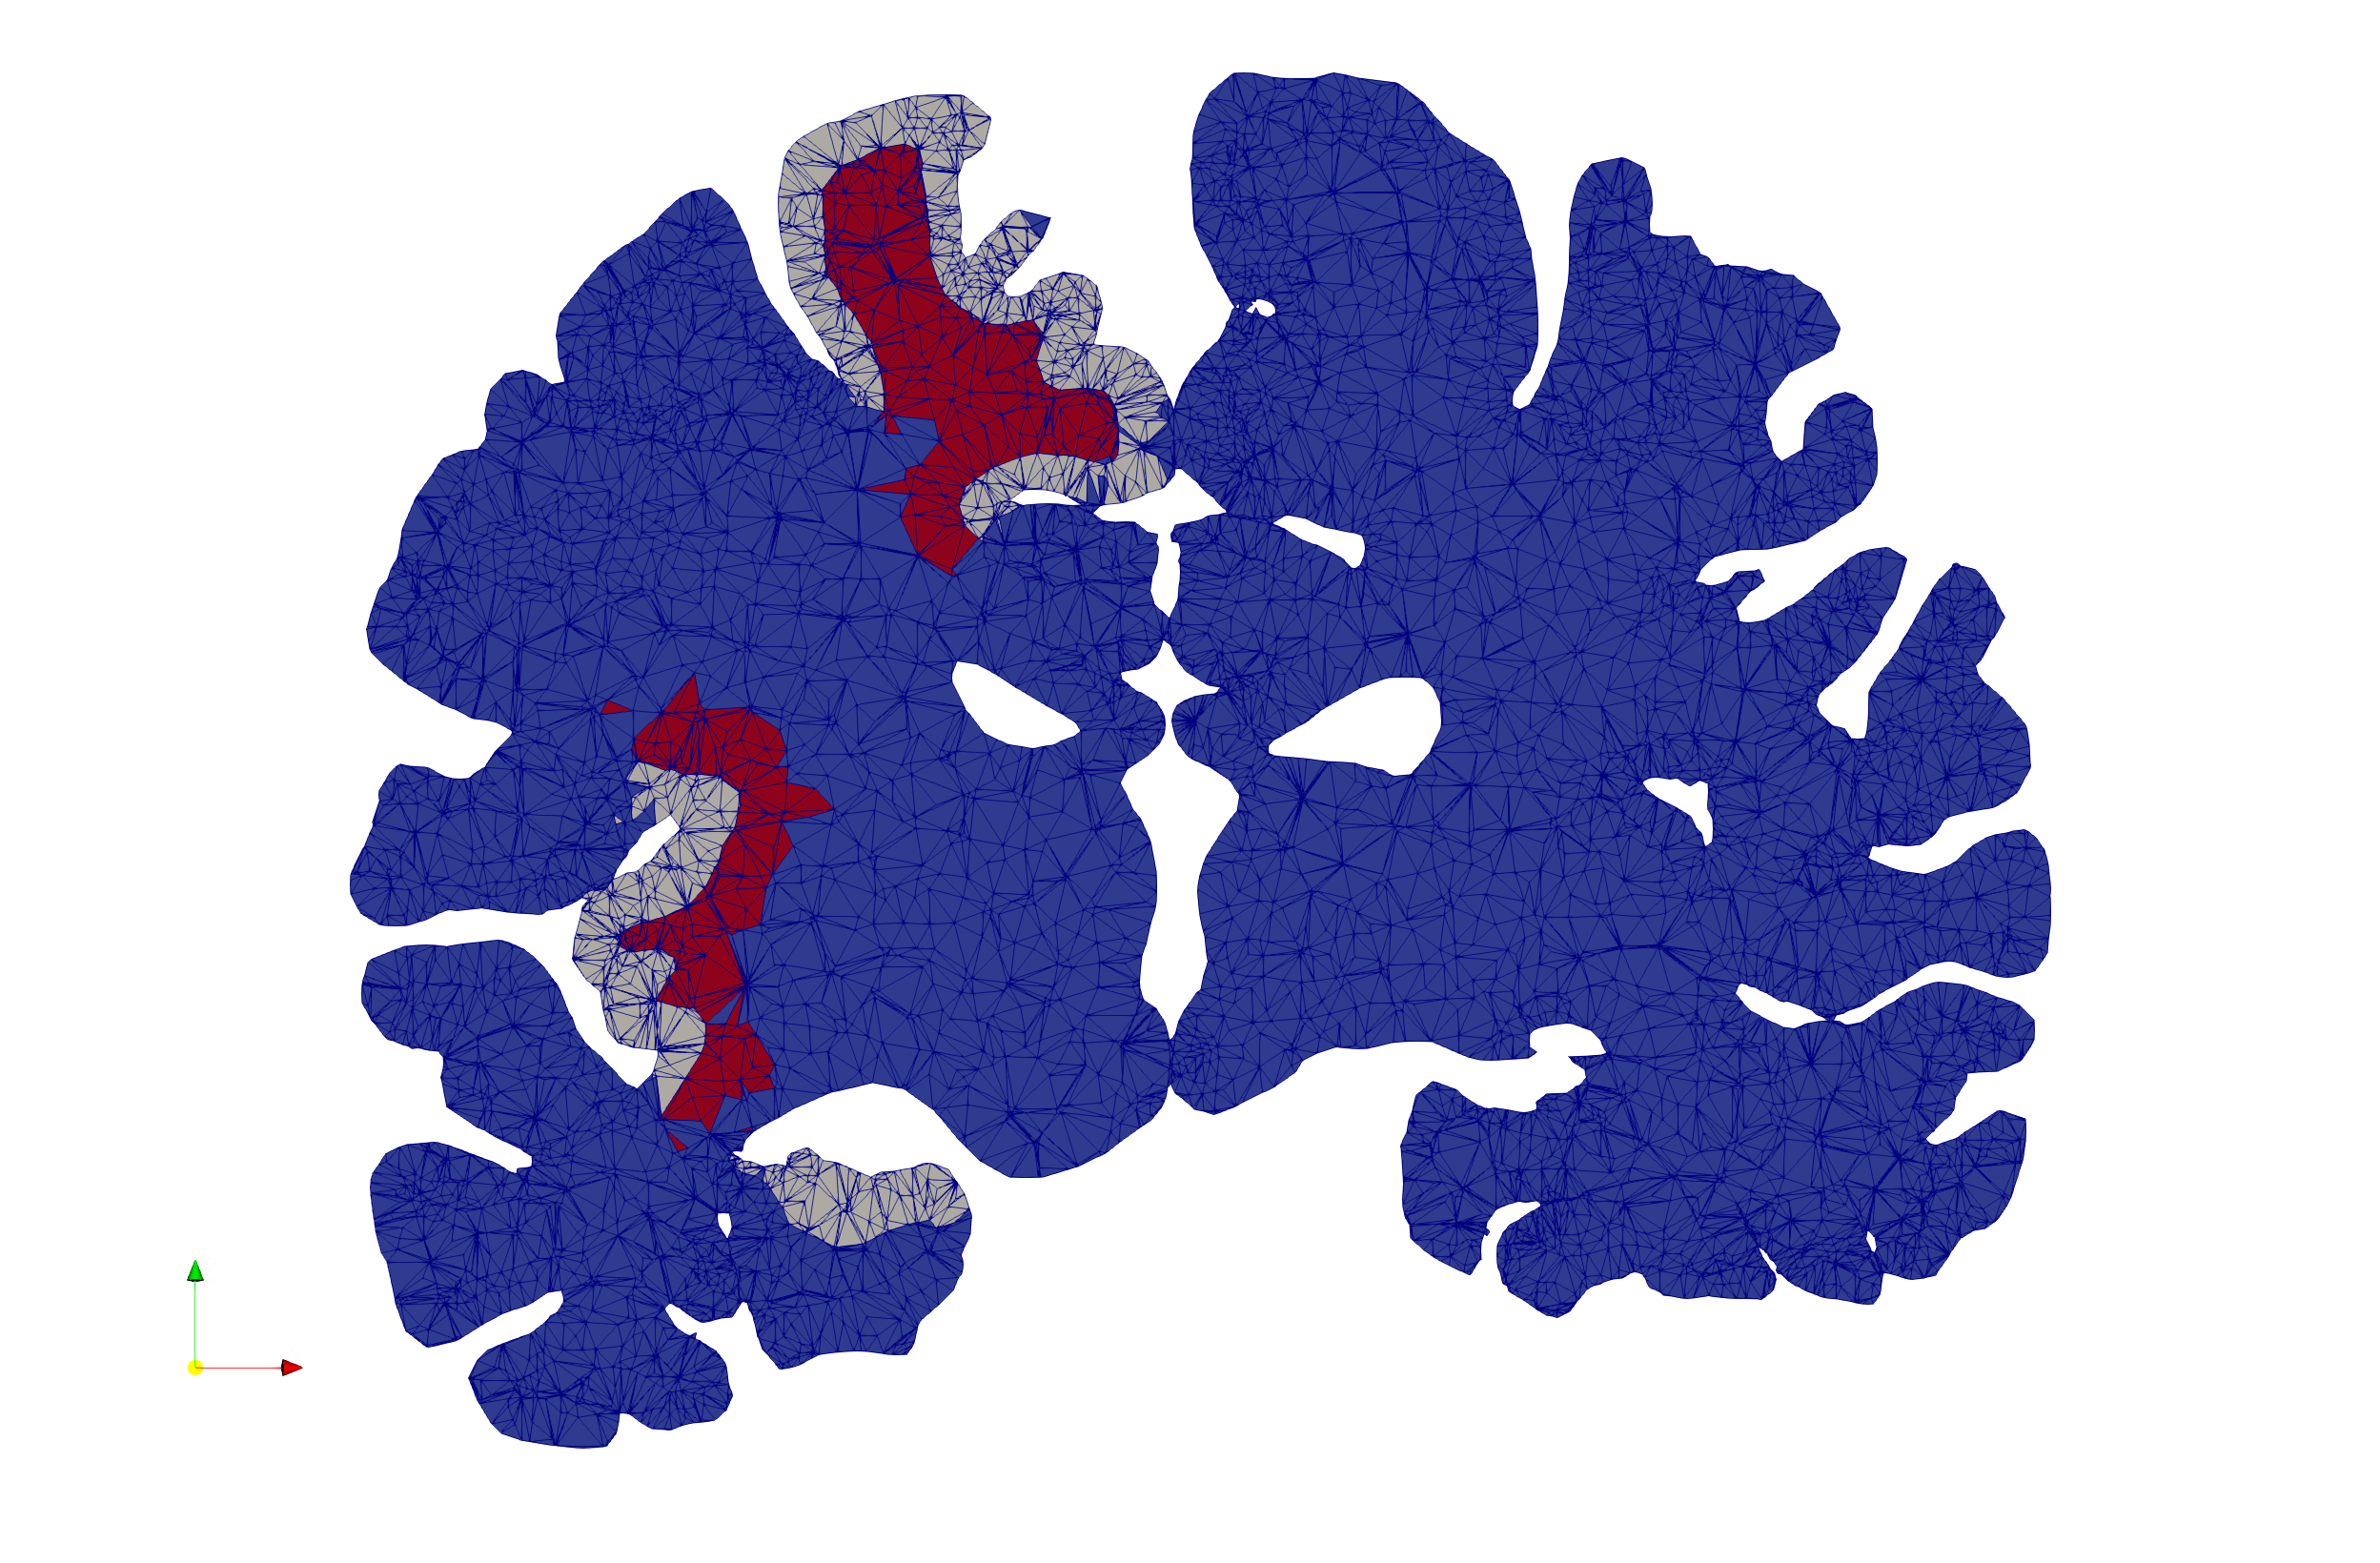
\includegraphics[width=0.49\textwidth]{./graphics/chp6/Gadovist_slice_subdomain.png}
%  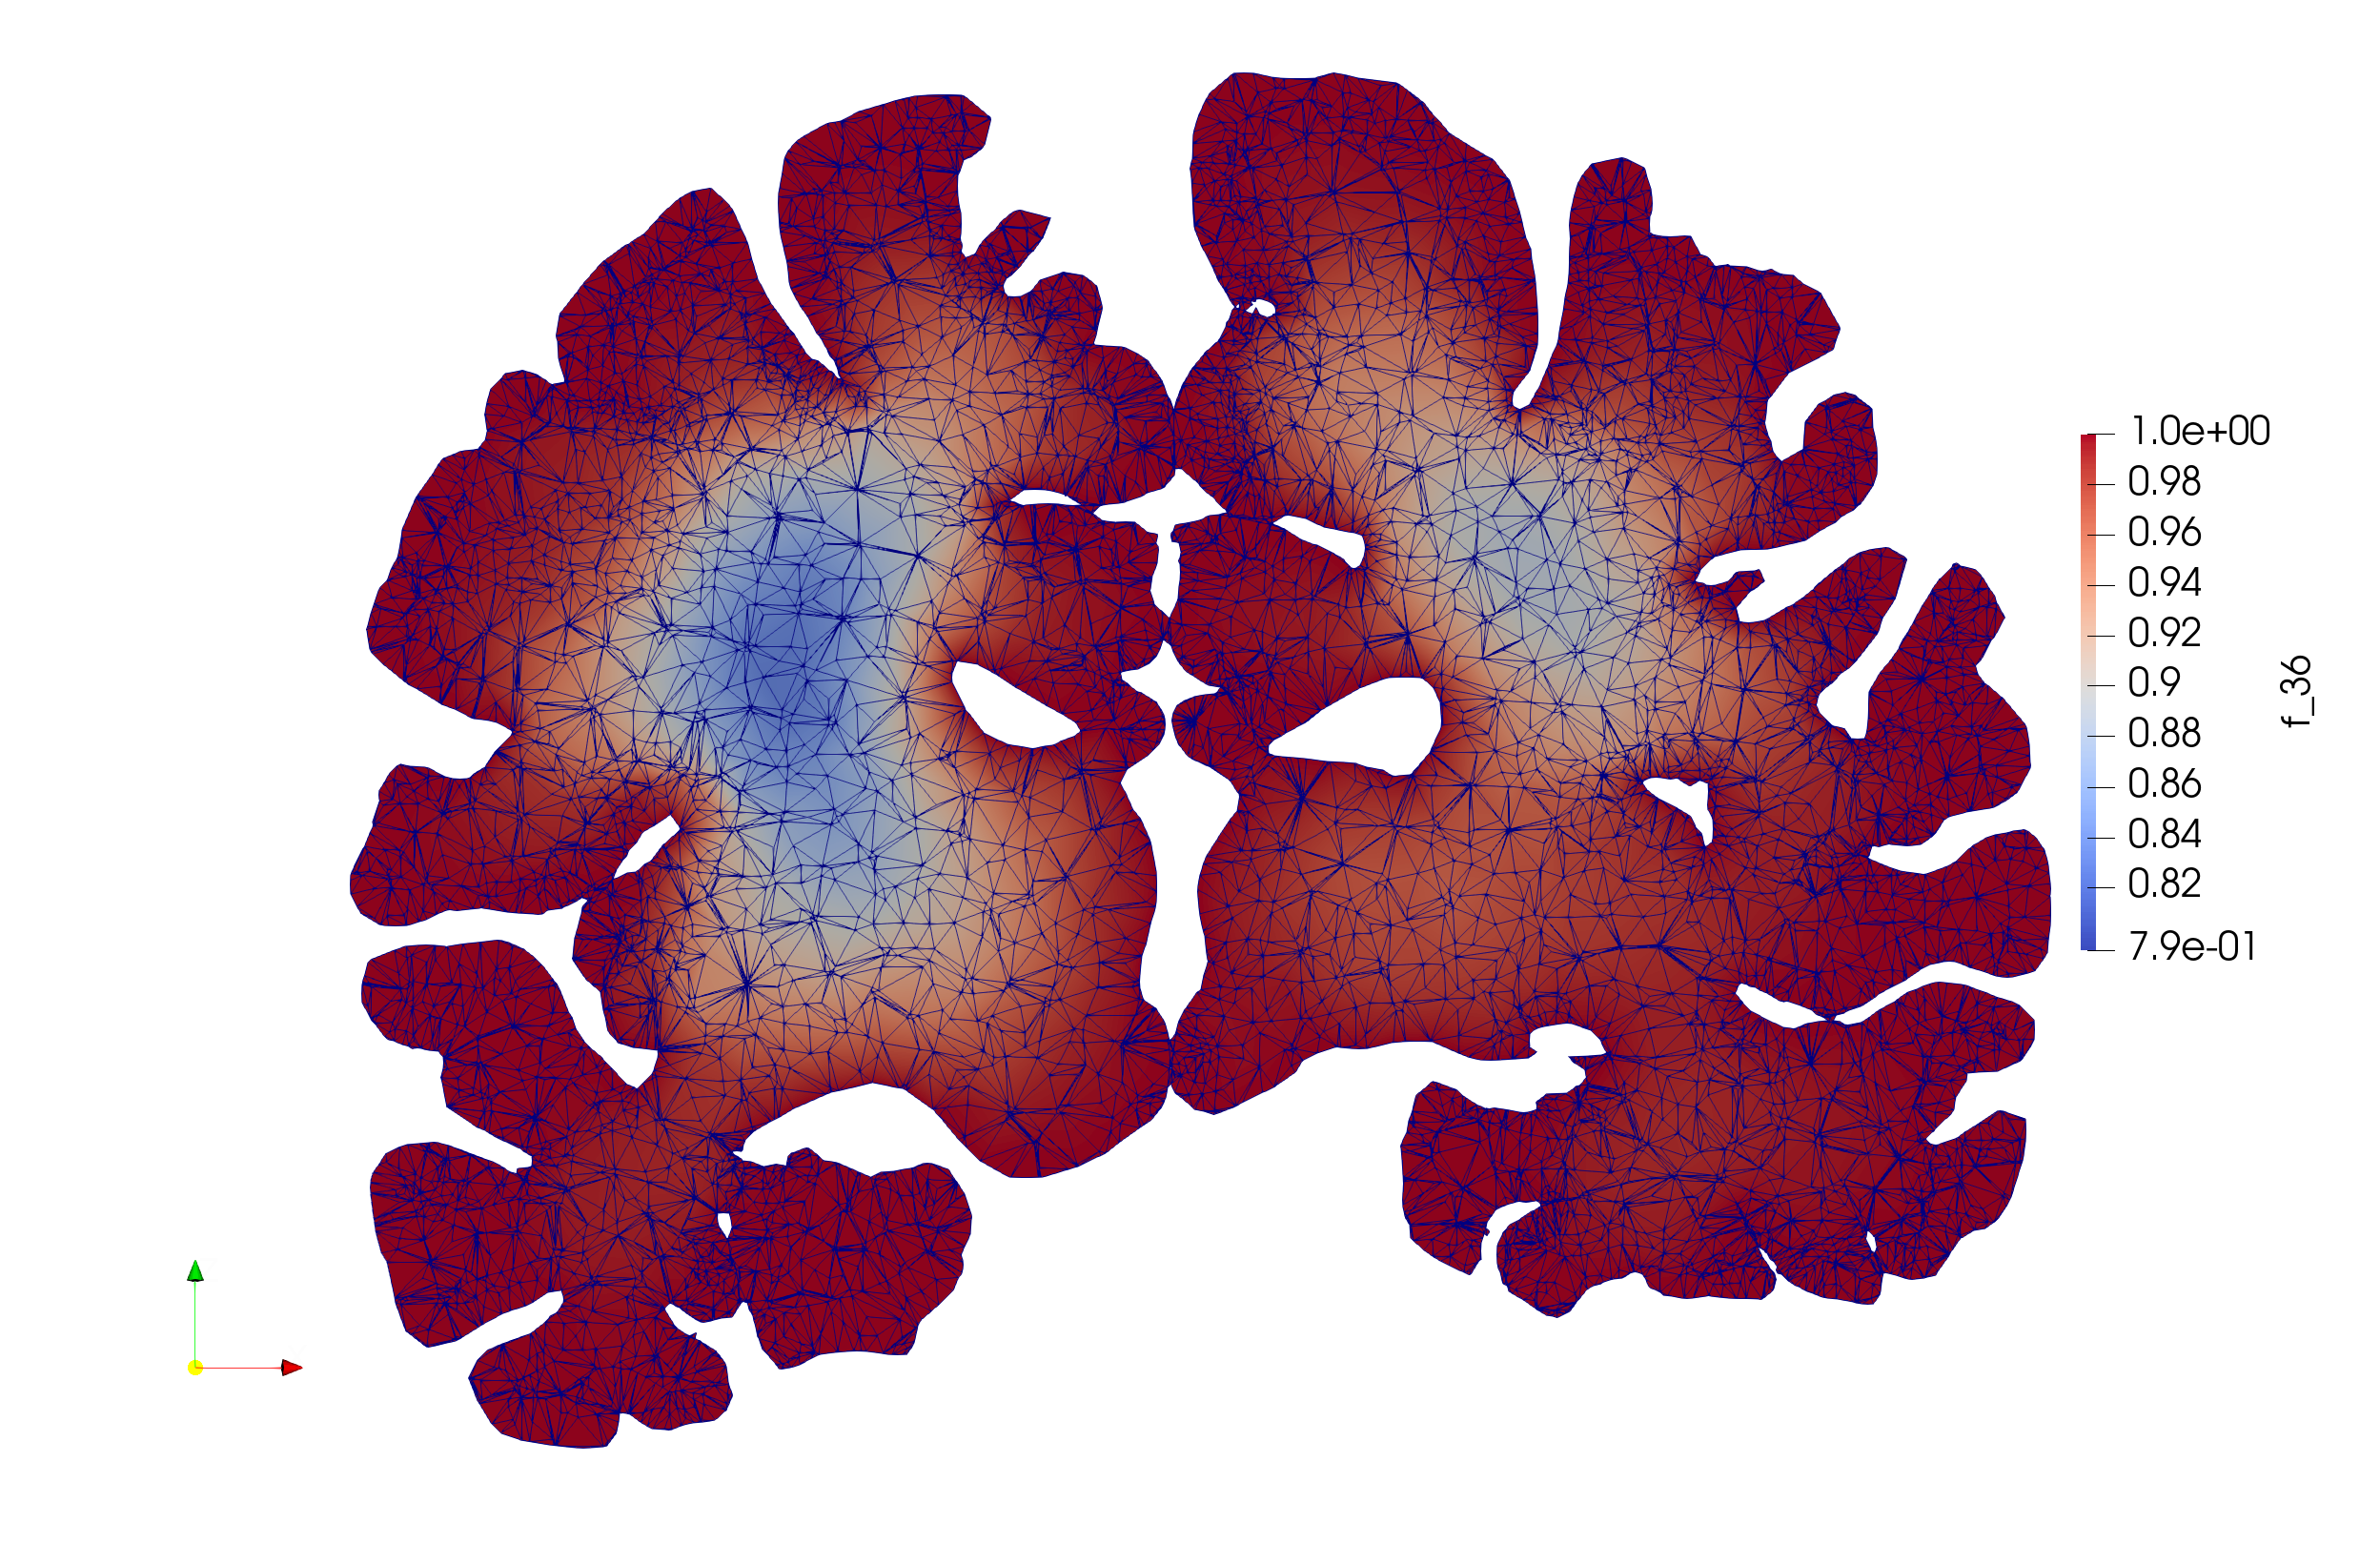
\includegraphics[width=0.49\textwidth]{./graphics/chp6/Gadovist_slice_9hours.png}
%  \caption{
%    The mesh and subdomains for the mesh with resolution parameter set to 32 (left)  
%    and the simulated distribution of Gadobutrol after 
%    9 hours (right).}
%  \label{fig:chp6:numerics4}
%\end{figure}

\begin{figure}	
  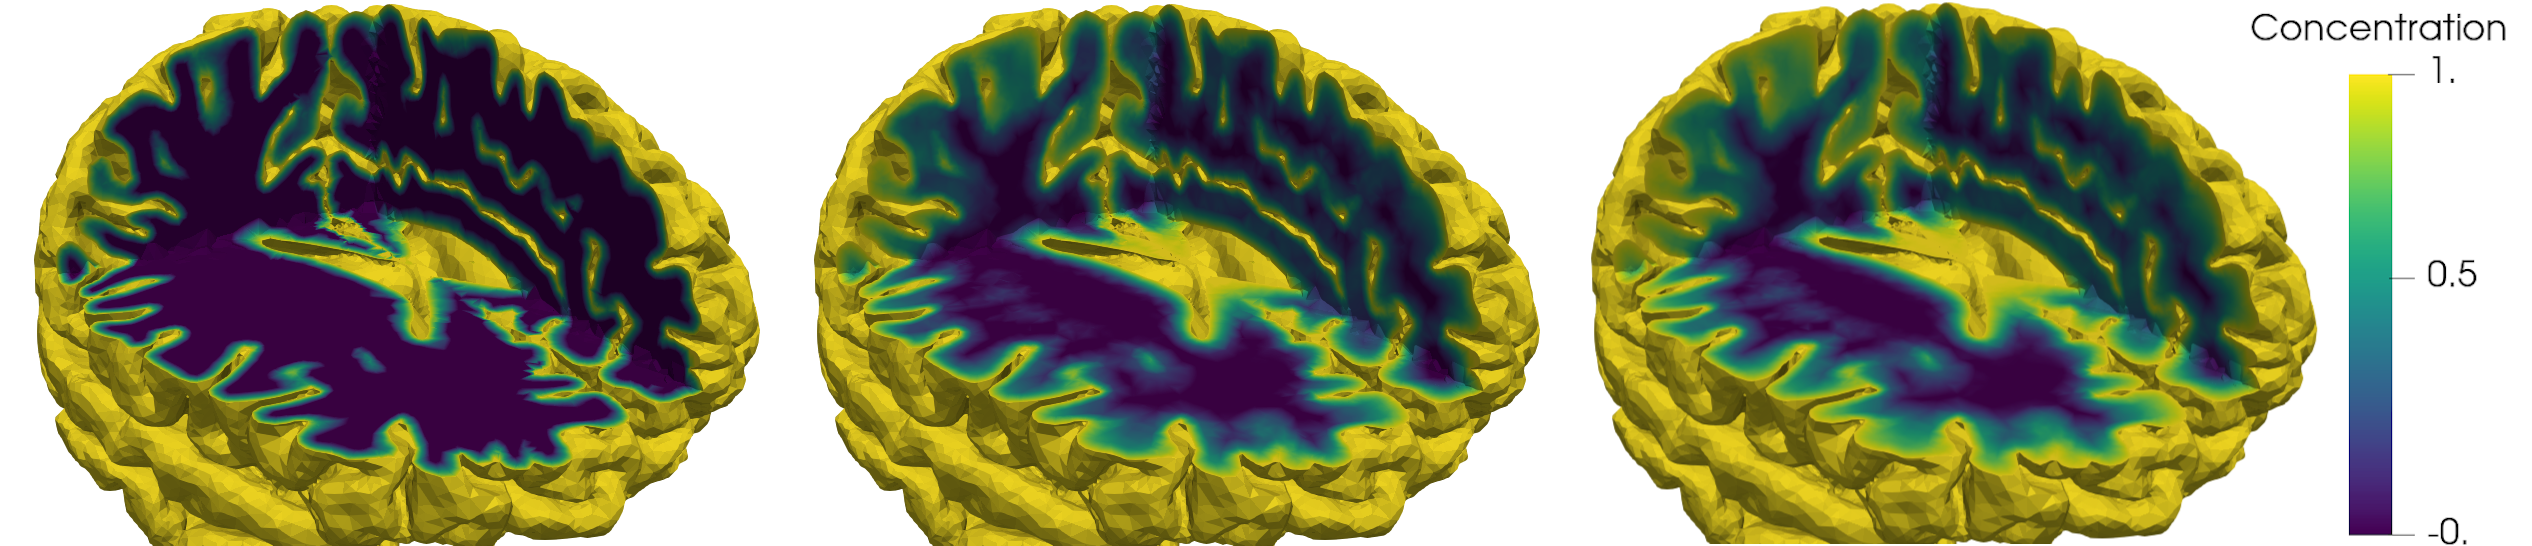
\includegraphics[width=0.98\textwidth]{./graphics/chp6/Image1.png}
  \caption{
    The simulated distribution of gadobutrol, for a mesh with resolution parameter set to 32, after 0 hours (left), %
    after 5 hours (middle) and after 9 hours (right).}
  \label{fig:chp6:numerics4}
\end{figure}
\begin{figure}	
  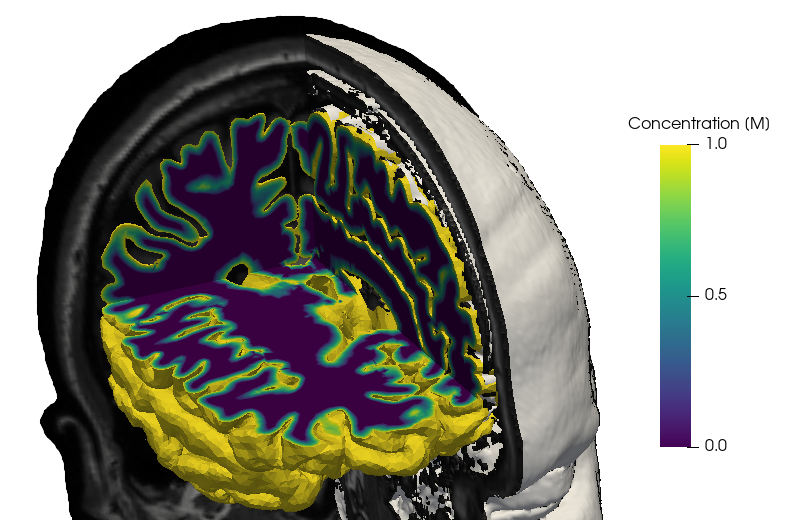
\includegraphics[width=0.90\textwidth]{./graphics/chp6/Image2.png}
  \caption{Illustration of the simulated distribution of solute
    concentration in the brain within the cranium.}
  \label{fig:chp6:numerics5}
\end{figure}



\subsection{Accuracy and convergence of computed quantities} 

\index{mesh convergence}
A common question and topic in numerical simulations is whether the
computed solutions have converged.  We therefore investigate next the mesh
convergence of the standard Galerkin and mass-lumped Galerkin
approaches. More precisely, we consider a set of meshes, aiming to 
determine the 
%
%of increasing
%resolution and compare the quantities computed on the different meshes
%aiming for determining 
accuracy of the numerical solution. In this
example, we consider a roughly uniform refinement, but the mesh is not
refined in place; rather, a sequence of meshes is first generated at
different resolutions using the surface volume meshing toolkit (\svmtk). In particular, 
we construct a sequence of quasi-uniform meshes, as follows (using 
\emp{mri2fem/chp6/create\_mesh\_refinements.py}):
\index{mesh refinement!uniform}
\newpythonsnippet{chp6}{create_mesh_refinements.py}{0}{100}

After creating the meshes we mark the subdomains of interest and map the DTI data onto the mesh, before 
running the simulations. The following is a code snippet from \emp{mri2fem/chp6/all.sh} that shows how
the 16 mesh is created by the scripts described in the previous chapters: 
\begin{lstlisting}[style=bashStyle]
# using the 16 mesh 
# convert to h5
python3 ../chp4/convert_to_dolfin_mesh.py \
   --meshfile brain_16.mesh --hdf5file brain_16.h5

# mark subdomains  
python3 ../chp4/add_parcellations.py \
    --in_hdf5 brain_16.h5 \
   --in_parc ../chp4/wmparc.mgz \
   --out_hdf5 brain_16_tags.h5 \
   --add 17 1028 1035 3028 3035

# add dti to the h5 file 
python3 ../chp5/dti_data_to_mesh.py  \
   --dti ../chp5/clean-dti.mgz \
   --mesh brain_16_tags.h5 --label 1 0.4 0.6 \
   --out DTI_16.h5 

# run simulation 
python3 chp6-diffusion-mritracer.py --mesh DTI_16.h5 \
   --lumped lumped --label uniform16lumped 
python3 chp6-diffusion-mritracer.py --mesh DTI_16.h5 \
   --lumped not --label uniform16notlumped 
\end{lstlisting}


The average gadobutrol concentrations in the hippocampus over time
for the sequence of meshes generated here are shown in
Figure~\ref{fig:chp6:numerics2}, with (right) and without (left)
mass lumping. Clearly, the standard Galerkin approach (left) seems to
yield more consistent results than the mass-lumped Galerkin scheme
(right). However, even for the standard Galerkin scheme, whether the
solutions are fully converged  seems questionable at the highest
resolution tested (around 15.5 million mesh cells). Recall that piecewise
constants are used to represent the anisotropic diffusion tensor $D$.
This DG construction requires about nine entries per cell, thus yielding
approximately 140 million values for 15.5 million cells. Higher resolutions, such
as those for piecewise linear or quadratic constructions, are not
feasible on a personal computing device with only 32 gigabytes of RAM.
\begin{figure}	
  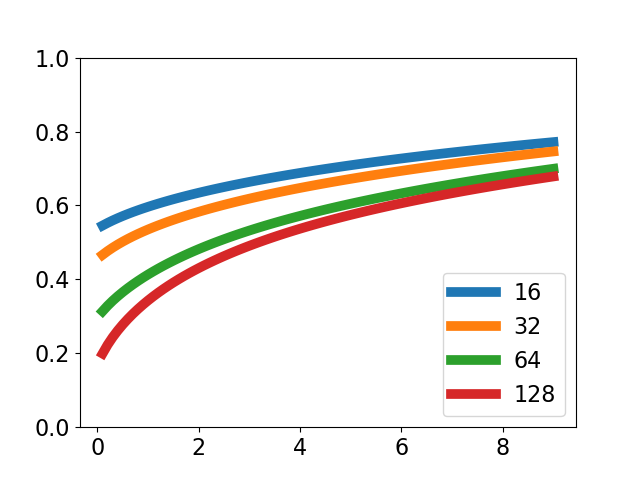
\includegraphics[width=0.49\textwidth]{./graphics/chp6/tracer_hippocampus_uniform_notlump.png}
  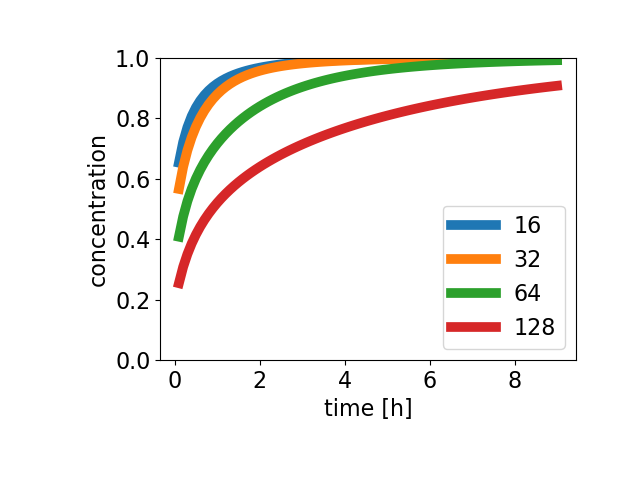
\includegraphics[width=0.49\textwidth]{./graphics/chp6/tracer_hippocampus_uniform_lump.png}
  \caption{Average gadobutrol concentration in the hippocampus (y-axis,
    arbitrary unit) versus time (x-axis, hours) for different mesh
    resolutions, $\Delta t = 6$ min. Quasi-uniform mesh sequence with
    $N=16$, $32$, $64$, $128$ generated by \svmtk. Standard Galerkin (left)
    versus mass-lumped Galerkin (right) discretizations.}
\label{fig:chp6:numerics2}
\end{figure}

\index{mesh refinement!adaptive}
To further assess the accuracy and convergence of the computed
concentrations under mesh refinements, we therefore also consider
adaptively refined meshes. In particular, we focus on the hippocampus
and adaptively refine the meshes in this region, starting from the
$N=16$ brain mesh of the previous mesh sequence. Again, we plot the
average gadobutrol concentrations in the hippocampus over time for
a sequence of adaptively refined meshes (see
Figure~\ref{fig:chp6:numerics3} with (right) and without (left)
mass-lumping). Using this technique, we find the solutions between the second,
third, and fourth adaptive refinements differ little for the standard
scheme. However, mesh convergence for the mass-lumped Galerkin
strategy remains unclear, even after four refinements to the
hippocampal region. Finally, looking at the mesh statistics (number of
vertices, cells, and range of mesh sizes) for the uniformly and
adaptively refined meshes (Tables~\ref{tab:uniref} and
\ref{tab:localref}), we note that the actual $h$ required for mesh
convergence is around two to ten times smaller than our initial estimate
(Section~\ref{sec:chp6:1D-tests}).
\begin{figure}	
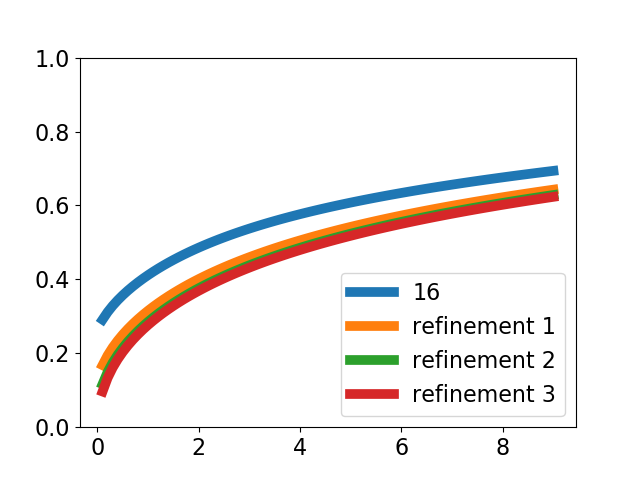
\includegraphics[width=0.49\textwidth]{./graphics/chp6/tracer_hippocampus_notlumped_addaptive.png}
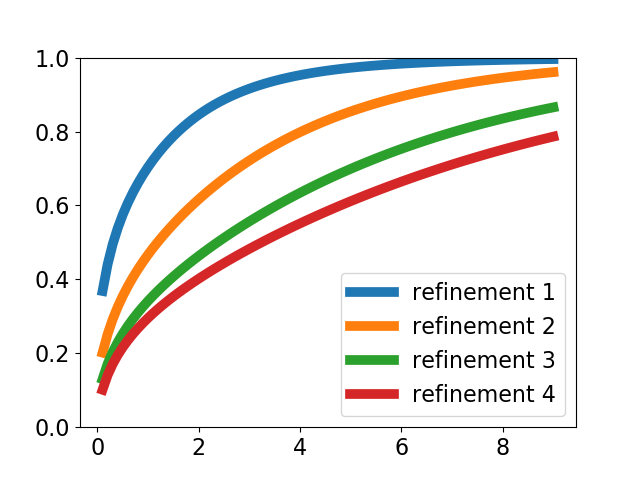
\includegraphics[width=0.49\textwidth]{./graphics/chp6/tracer_hippocampus_lumped_addaptive.png}
  \caption{Average gadobutrol concentration in the hippocampus
    (y-axis, arbitrary unit) versus time (x-axis, hours) for a
    sequence of adaptively refined meshes, $\Delta t = 6$
    minutes. Standard Galerkin (left) versus mass-lumped Galerkin (right)
    discretizations.}
\label{fig:chp6:numerics3}
\end{figure}
\begin{table}%
  \label{chp6:meshstat}
  \centering
  \begin{minipage}{.45\textwidth}%
    \begin{tabular}{l|cccc}
      Refinement & Vertices & Cells  & $h_{\min}$ & $h_{\max}$ \\ \hline
      16 & 94K & 457K & 0.97 & 11.4 \\  
      32 & 194K & 908K &  0.46 & 5.7 \\  
      64 & 567K &  2.75M & 0.26 & 2.9 \\
      128 &  2.8M & 15.5M &  0.14 & 1.45
    \end{tabular}
    \label{tab:uniref}
  \end{minipage}%
  \hspace{2em}
  \begin{minipage}{.45\textwidth}%
    \begin{tabular}{c|cccc}
	    Refinement & Vertices & Cells & $h_{\min}$ & $h_{\max}$ \\ \hline
	     1 & 99K &  479K &  0.64 &  11.4 \\
	     2 & 123K& 613K & 0.30 &  11.4 \\
	     3 & 275K &  1.5M  &  0.14 & 11.4 \\
	     4 & 1.3M &  7.7M  & 0.07 &  11.4 \\
    \end{tabular}
    \label{tab:localref}
  \end{minipage}%
  \caption{Mesh statistics (number of vertices, cells, and minimal and
    maximal cell sizes) for the (left) uniformly refined and
    (right) adaptively refined mesh sequences.}
\end{table}
